\documentclass[12pt]{article}

\title{CRPL: Architecture}
\author{Harrison Beau Barker}

\usepackage{graphicx}
\graphicspath{ {images/} }

\begin{document}
	\maketitle
	
	\section{.NET service architecture}
	
	\begin{description}
		\item[Auth service] user authentication.
			\begin{enumerate}
				\item Auth
			\end{enumerate}
		\item[Wallet service] user ethereum wallet/account management.
			\begin{enumerate}
				\item CRUD
			\end{enumerate}
		\item[Issuing service] registering new copyrights to the blockchain.
			\begin{enumerate}
				\item Register
			\end{enumerate}
		\item[Verification service] verifying the authenticity and originality of a work.
			\begin{enumerate}
				\item VerifyWork
				\item Hash
				\item SignWork (maybe in the issuing)
			\end{enumerate}
		\item[General query service] querying the whole system mainly used for UI, copyright index and search.
			\begin{enumerate}
				\item Get all
				\item Search
				\item Get my work
				\item Get work
			\end{enumerate}
		\item[Rights management service] modification, transfer of ownership.
			\begin{enumerate}
				\item Transfer ownership
				\item UnRegister
				\item ConvertRights
			\end{enumerate}
		\item[Dispute service] filing and resolving copyright disputes.
			\begin{enumerate}
				\item FileDispute
				\item Resolve
				\item Cancel
			\end{enumerate}
		\item[Contract management] deployment and monitoring of systems contracts
		\item[Ping service] work "use" tracking
			\begin{enumerate}
				\item Ping
				\item GetPings
			\end{enumerate}
	\end{description}
	
	\begin{description}
		\item[Payment distribution service]	
	\end{description}

	\section{API}
	
	\begin{itemize}
		\item /user
			\begin{description}
				\item [GET] /auth
				\item [CRUD] /wallet
			\end{description}
		\item /cpy
			\begin{description}
				\item [POST] /submit/\#application-id (mint once the application has been accepted)
			\end{description}
		\item /forms (all applications and forms)
			\begin{description}
				\item [GET] /\#application-id
				\item [DELETE] /\#application-id
				\item [GET] /all
				\item [POST] /cpy/register
				\item [POST] /cpy/unregister
				\item [POST] /cpy/transfer
				\item [POST] /cpy/convert (convert copyright type)
				\item [POST] /dispute/file
				\item [POST] /dispute/resolve
			\end{description}
		\item /work
			\begin{description}
				\item [POST] /upload
			\end{description}
		\item /q
			\begin{description}
				\item [GET] /\#id
				\item [GET] /all
				\item [GET] /search
				\item [GET] /me
				\item [GET] /\#id/work (users work)
			\end{description}
		\item /dispute
			\begin{description}
				\item [POST] /file/\#application-id (submit application)
				\item [POST] /resolve/\#application-id (submit application)
				\item [DELETE] /cancel/\#id
			\end{description}
		\item /p

	\end{itemize}
	
	\section{Copyright smart contract}
	
	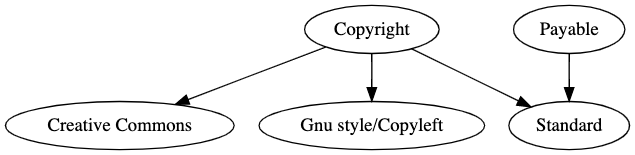
\includegraphics[scale=0.5]{sc.png}
	
	\section{Database}
	
	\section{Angular}
	
	\section{Copyright registration flow}
	
	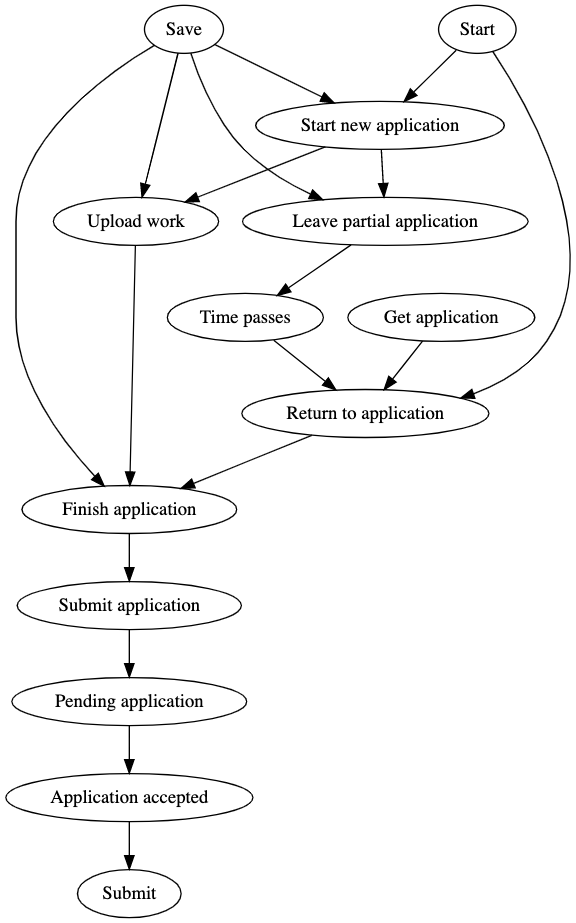
\includegraphics[scale=0.5]{reg.png}
	
\end{document}